\documentclass[10pt,a4paper]{article}
\usepackage[margin=2.2cm]{geometry}
\usepackage{fontspec}
\usepackage{kotex}
\setmainfont{Apple SD Gothic Neo}
\setsansfont{Apple SD Gothic Neo}
\usepackage{amsmath,amssymb}
\usepackage{graphicx}
\usepackage{caption}
\usepackage[dvipsnames]{xcolor}
\usepackage[colorlinks=true,linkcolor=MidnightBlue,citecolor=MidnightBlue,
            urlcolor=MidnightBlue]{hyperref}
\usepackage{titlesec}
\titleformat{\section}{\large\bfseries}{\thesection}{0.6em}{}
\captionsetup{font=small,labelfont=bf}
\setlength{\parskip}{0.35em}
\setlength{\parindent}{0pt}
\usepackage{mdframed}
\newmdenv[linewidth=0.4pt,linecolor=gray!60,backgroundcolor=gray!5,
          innertopmargin=6pt,innerbottommargin=6pt,skipabove=8pt,skipbelow=8pt]{claimbox}
\newcommand{\claim}[2]{\begin{claimbox}\textbf{주장.} #1\par\smallskip
  \textcolor{gray!70}{\textbf{반증 조건.} #2}\end{claimbox}}

\title{\bfseries 왕국은 없었다\\[2pt]
\large 아이돌 챌린저 `한 왕국 간발'의 강등 --- $828$ 보류 판정의 완결}
\author{월드모델 실험실 · 노트 $859$}
\date{2026-08-08}
\begin{document}\maketitle

\section{한 줄}

$828$ 이 보류로 걸어 둔 판정 — `아이돌에선 TabPFN 챌린저가 챔피언을 이긴다
(하한 $+0.0082$ · 간발)' — 을 소속사 군집 자로 완결했다. 별칭표 v$1$ 을
부트 실행 \textbf{전에} 동결하고(플레디스 영↔한 병합 등 · 부트 후 병합 추가
금지), $828$ 챌린저 팔을 재현($\Delta$ $+0.1616$ 대 기록 $+0.1732$ · 차
$0.012$)한 뒤 행별 벡터를 동결하고, 군집 부트 BCa($45/51$ 군집 · B$=$$10{,}000$)
로 다시 쟀다: \textbf{CI $[-0.0035, +0.3624]$ --- $0$ 을 문다. 판정 불능
강등.} 무군집 재실행도 하한 $+0.0001$(끝점 몬테카를로 오차 안 · 정전화
금지), percentile 자로도 양쪽 다 $0$ 을 문다 --- \textbf{강등이 자 종류
무관으로 강건하다.}

\begin{figure}[t]\centering
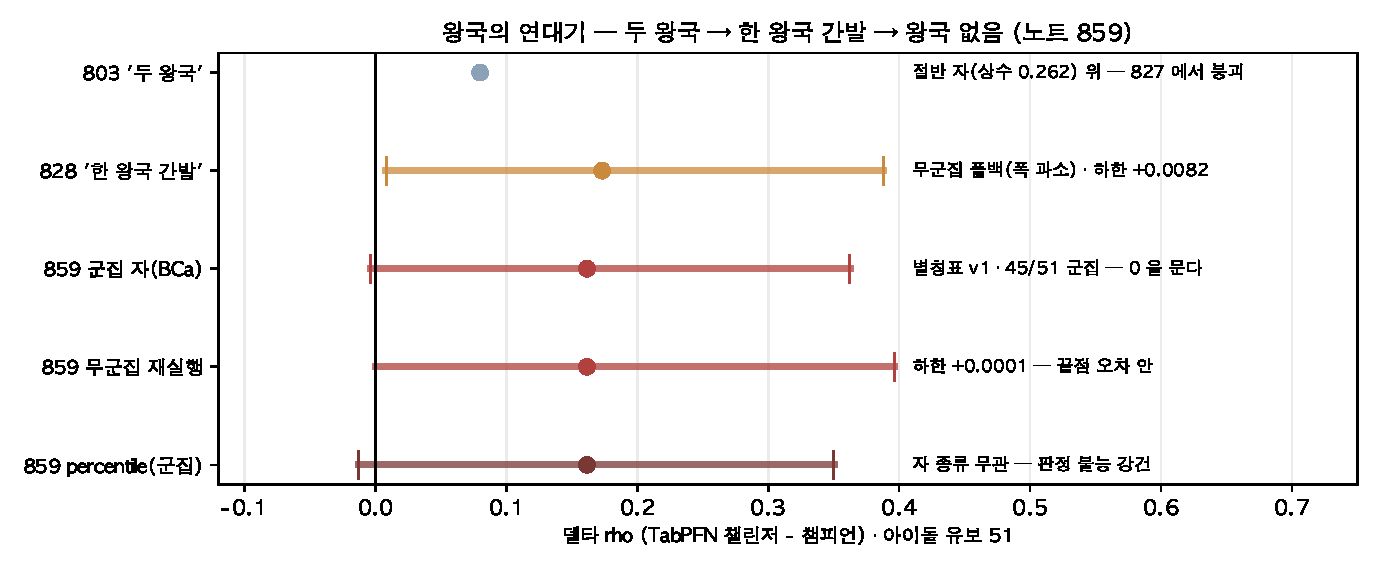
\includegraphics[width=0.97\textwidth]{figs/nokingdom.pdf}
\caption{왕국의 연대기 --- 구간이 정직해질수록 왕국이 줄었다.}
\end{figure}

\claim{\textbf{T$1$ 구역별 분업의 서사 정정: 두 왕국($803$) $\to$ 한 왕국
간발($828$) $\to$ 왕국 없음($859$).} 아이돌 챌린저 라우팅(TabPFN 보조 헤드)의
근거가 소멸했다 --- 승격 절차 폐기 · 챔피언 유지 기본. 점추정 $+0.16$ 은
남지만 유보 $51$행으로는 판정이 서지 않는다 --- 재개 조건: 아이돌 유보
$\sim2$배. 사전등록 갈래 d(군집 폭 $0.924$배 --- 축소)도 발동했는데
percentile 병기로 재현돼 \textbf{구현 오류가 아니라 자료 성질}(다건 군집
기여의 부분 상쇄)로 판정됐다.}
{강등의 몫 분해를 정직하게: $0$단계 점추정이 $828$ 대비 $-0.0116$
이동(자료 드리프트)했고 무군집 하한도 $+0.0082 \to +0.0001$ 로 내려갔다 ---
강등의 주역은 군집 자가 아니라 \textbf{간발 자체의 취약성}이다(군집 $45/51$
은 사전 병기한 구조적 상한대로 교정력이 작았다). 내 최빈 예측(하한 $0$
물기 $55\%$)이 적중했고 폭 방향($75\%$)은 미스 --- $3/4$.}

\section{부수}

lab/router.py 이행 --- 서빙 라우팅의 실행 주체(무정체 기본값 · names 등록
의무 · `만화' 정체 금지 · selftest). rescore$828$ 의 휘발 경로 수리. 티처
\#$24$ 자백 둘 반영($858$ normtest 는 동어반복 --- 채점 $2/3 \to$ 실질
$1/2$ 재채점 · dryrun 은 동결 채점기 실코드 미통과 --- harvest$844$c 로
등록). GitHub 흐름 $16$회째. 판 $\rho$ $0.4710$ 그대로.

\end{document}
